% -*- TeX:de -*-
\NeedsTeXFormat{LaTeX2e}
\documentclass[12pt,a4paper,titlepage]{article}

%\usepackage[ngerman]{babel} % german text
\usepackage[DIV12]{typearea} % size of printable area
\usepackage[T1]{fontenc} % font encoding
\usepackage[utf8]{inputenc} % probably on Linux

\usepackage{graphicx} % to include images
\usepackage{subfigure} % for creating subfigures
\usepackage{amsmath} % a bunch of symbols
\usepackage{amssymb} % even more symbols
\usepackage{booktabs} % pretty tables
\usepackage{csquotes}

% a floating environment for circuits
\usepackage{float}
\usepackage{caption}

\newfloat{circuit}{tbph}{circuits}
\floatname{circuit}{Schaltplan}

% a floating environment for diagrams
\newfloat{diagram}{tbph}{diagrams}
\floatname{diagram}{Diagramm}

\renewcommand{\familydefault}{\sfdefault} % activate to use sans-serif font as default

\sloppy % friendly typesettings

\usepackage{eurosym}
\usepackage{makeidx}
\usepackage{amsfonts}
\usepackage{mparhack}
\usepackage{array}
\usepackage{tabularx}
\usepackage{minitoc}
\usepackage[colorlinks=true]{hyperref}
\usepackage{epstopdf}
\usepackage{setspace}
\usepackage{csquotes}

\usepackage{float}
\usepackage{circuitikz}

\ctikzset{voltage/distance from line=.5}

\begin{document}

%%%%%%%%%%%%%%%%%%%%%%%%%%%%%%%%
% create title page
%%%%%%%%%%%%%%%%%%%%%%%%%%%%%%%%

\begin{titlepage}

\begin{figure*}[h!]
  
\includegraphics[width=8cm]{TULogo_CMYK}
\end{figure*}

\begin{center}
\vspace*{1.3cm}
{\Huge Elektrotechnische Grundlagen der Informatik\\(LU 182.692)\\}
\vspace{1.7cm}
{\LARGE Protokoll der 1. Laborübung: \enquote{Messtechnik}\\}
\vspace{1.7cm}

% fill in group number and date of lab here
% CHANGE ME!
{\Large Gruppennr.: 22 \hspace{1cm} Datum der Laborübung: 04.05.2017}

% fill in IDs and names here
% CHANGE ME!
\begin{table}[h!]
\centering
\begin{tabular}{|p{3.5cm}|p{3.5cm}|p{6.5cm}|}
\hline \textbf{Matr. Nr.} & \textbf{Kennzahl} & \textbf{Name} \\
\hline
& & \\
\hline
1614835 & & Jan Nausner \\
\hline
& & \\
\hline
\end{tabular}
\end{table}

\end{center}
\vspace{1.0cm}

\begin{table}[h!]
\begin{tabular}{|l|l|}
\hline \textbf{Kontrolle} & \checkmark \\
\hline stromrichtige Messschaltung & \\
\hline spannungsrichtige Schaltung & \\
\hline Spannungs- Stromteilerschaltung & \\
\hline Superpositionsprinzip & \\
\hline Arbitrary Waveforms & \\
\hline Diodenkennlinie & \\
\hline
\end{tabular}
\end{table}

\end{titlepage}

%%%%%%%%%%%%%%%%%%%%%%%%%%%%%%%%
% start of actual document
%%%%%%%%%%%%%%%%%%%%%%%%%%%%%%%%

\newpage

\setcounter{page}{2}

\section{Innenwiderstand der Messgeräte}

\subsection{Aufgabenstellung}
In dieser Messung müssen die Innenwiderstände der verwendeten Messgeräte durch geeignete Aufbauten bestimmt werden.

\subsection{Innenwiderstand des Amperemeters}

\subsubsection{Verwendete Materialien und Einstellungen:}
\begin{itemize}
  \item Netzteil: Agilent U8031A
  \item Versorgungsspannung: $1V$
  \item Amperemeter: Amprobe 37XR-A
  \item Voltmeter: Amprobe 37XR-A
  \item Vorwiderstand: $1k\Omega$ (gemessen $0,983k\Omega$), $P_{tot} = \frac{1}{4}W$
\end{itemize}

\subsubsection{Schaltungsaufbau}
\begin{figure}[H]
  \centering
  \begin{circuitikz}[european] \draw
    (-0.2,0) -- (0.2,0)
    (0,0) to[V, v<=$U_Q$] (0,2)
    to[R, l=$1k\Omega$] (2,2)
    to[ammeter, i_=$I_A$, *-*, v^>=$U_A$] (6,2)
    (2,2) -- (2,0) to[voltmeter] (6,0) -- (6,2)
    (6,2) -- (6.5,2)
    (6.5,1.8) -- (6.5,2.2);
  \end{circuitikz}
  \caption{Messung $R_A$}
\end{figure}

\subsubsection{Durchführung}
Das Amperemeter wird in Serie zu dem Vorwiderstand (zur Begrenzung des Stroms) geschalten und das Voltmeter parallel zum Amperemeter. An die gesamte Schaltung wird eine Spannung von $1V$ angelegt. Mit dem Voltmeter wird der Spannungsabfall am Amperemeter und mit dem Amperemeter der fließende Strom für die jeweiligen Messbereiche gemessen.

\subsubsection{Ergebnis}
\begin{table}[H]
  \centering
  \begin{tabular}{c|c|c}
    $U_Q$ & $I_A$ & $U_A$ \\
    \hline
    $1V$ & $504,3\mu A$ & $503,3mV$ \\
    \hline
    $5V$ & $5,013mA$ & $56,4mV$ \\
    \hline
    $20V$ & $0,022A$ & $0,7mV$
  \end{tabular}
  \caption{Gemessene Werte}
\end{table}

\noindent Der Innenwiderstand $R_A$ des Amperemeters kann jetzt über das Ohmsche Gesetz berechnet werden: $R_A = \frac{U_A}{I_A}$.

\begin{table}[H]
  \centering
  \begin{tabular}{c|c}
  Messbereich & $R_A$ (gerundet) \\
  \hline
  $\mu A$ & $998\Omega$ \\
  \hline
  $mA$ & $11,25\Omega$ \\
  \hline
  $A$ & $0,032\Omega$
  \end{tabular}
  \caption{Innenwiderstände}
\end{table}

\noindent Der Innenwiderstand bei einem idealen Amperemeter wäre $R_A = 0\Omega$. Dieser Wert ist jedoch nicht zu erreichen, da dies einem Kurzschluss gleichkommen würde. Bei den verschiedenen Messbereichen werden verschiedene Widerstände benötigt, da z.B. bei kleinen Strömen meist große Widerstände zum Einsatz kommen, wohingegen bei großen Strömen die Widerstände meist klein sind. So wird sichergestellt, dass die Messergebnisse so gering wie möglich verfälscht werden. Trotzdem muss man sich bei Messungen der ohmschen Eigenschaft des Amperemeters und derer möglichen Auswirkungen bewusst sein.

\subsection{Innenwiderstand des Voltmeters}

\subsubsection{Verwendete Materialien und Einstellungen:}
\begin{itemize}
  \item Netzteil: Agilent U8031A
  \item Versorgungsspannung: $20V$
  \item Amperemeter: Amprobe 37XR-A
  \item Voltmeter: Amprobe 37XR-A
\end{itemize}

\subsubsection{Schaltungsaufbau}
\begin{figure}[H]
  \centering
  \begin{circuitikz}[european] \draw
    (0,0) -- (0,-0.5)
    (-0.2,-0.5) -- (0.2,-0.5)
    (0,0) to[V, v<=$U_Q$] (2,0)
    to[ammeter, i=$I_V$] (4,0)
    to[voltmeter] (6,0)
    (6,0) -- (6,-0.5)
    (5.8,-0.5) -- (6.2,-0.5);
  \end{circuitikz}
  \caption{Messung $R_V$}
\end{figure}

\subsubsection{Durchführung}
Das Amperemeter und das Voltmeter werden in Serie geschalten und an die gesamte Schaltung wird eine Spannung von $20V$ angelegt. Mit dem Amperemeter wird der fließende Strom gemessen. Das gewählte Voltmeter hat nur einen Messbereich.

\subsubsection{Ergebnis}
\begin{table}[H]
  \centering
  \begin{tabular}{c|c}
    $U_Q$ & $I_V$ \\
    \hline
    $20V$ & $2,25\mu A$
  \end{tabular}
  \caption{Gemessener Wert}
\end{table}

\noindent Der Innenwiderstand $R_V$ des Voltmeters kann jetzt über das Ohmsche Gesetz berechnet werden: $R_V = \frac{U}{I_V} = \frac{20V}{2,25\mu A} \approx 8,9M\Omega$

\noindent Der Innenwiderstand bei einem idealen Voltmeter wäre $R_V = \infty\Omega$. Dieser Wert ist jedoch nicht zu erreichen, da dies einer Unterbrechung gleichkommen würde. Bei Messungen muss man sich der ohmschen Eigenschaft des Voltmeters und derer möglichen Auswirkungen bewusst sein.

\section{Belastungsfehler}

\subsection{Aufgabenstellung}
Die Werte der gegebenen Widerstände sollen jeweils mittels sowohl spannungsrichtiger und stromrichtiger Schaltung als auch per Direktmessung mit dem Multimeter bestimmt werden. Weiters sollen die unterschiedlichen Messbereiche verwendet werden.

\subsection{Verwendete Materialien und Einstellungen:}
\begin{itemize}
  \item Netzteil: Agilent U8031A
  \item Amperemeter: Amprobe 37XR-A
  \item Voltmeter: Amprobe 37XR-A
  \item diverse Widerstände (siehe Tabelle)
\end{itemize}

\begin{figure}[H]
  \centering
  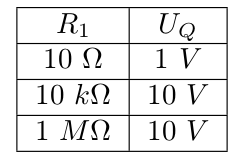
\includegraphics[width=40mm]{widerstandtabelle.png}
  \caption{Widerstände und Quellspannungen}
\end{figure}

\subsection{Schaltungsaufbau}

\begin{figure}[H]
  \centering
  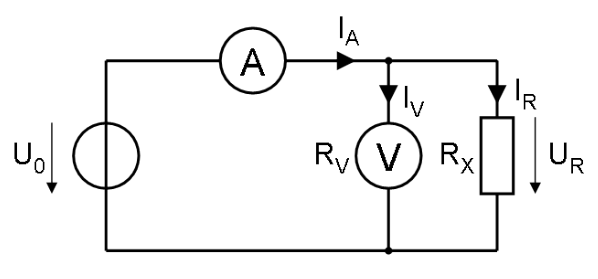
\includegraphics[width=100mm]{spannungsrichtig.png}
  \caption{Spannungsrichtige Messung}
\end{figure}

\begin{figure}[H]
  \centering
  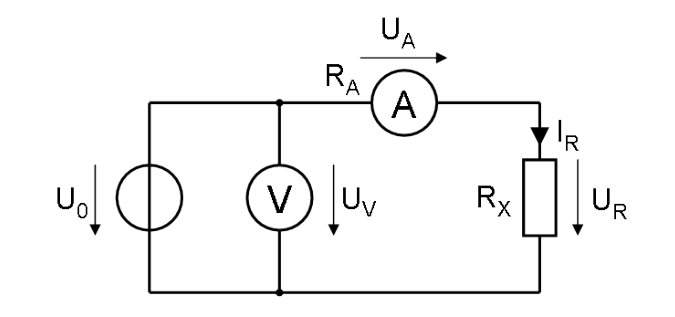
\includegraphics[width=100mm]{stromrichtig.png}
  \caption{Stromrichtige Messung}
\end{figure}


\subsection{Durchführung}
Es wird jeweils die Strom- bzw. Spannungsrichtige Schaltung aufgebaut. Für jeden Widerstand wird die jeweilige Quellspannung eingestellt, danach werden die Werte am Volt- und Amperemeter abgelesen (auch bei unterschiedlichen Messbereichen). Zum Schluss erfolgt noch eine Direktmessung der Widerstände mittels Ohmmeter.

\subsection{Ergebnis}
\begin{table}[H]
  \centering
  \begin{tabular}{c|c|c|c}
    $U_0$ & $R_1$ & $U_R$ & $I_A$ \\
    \hline
    $1V$ & $10\Omega$ & $454,2mV$ & $46,16mA$ \\
    \hline
    $1V$ & $10\Omega$ & $983,7mV$ & $0,1A$ \\
    \hline
    $10V$ & $10k\Omega$ & $9,062V$ & $924,9\mu A$ \\
    \hline
    $10V$ & $10k\Omega$ & $9,975V$ & $1,016mA$ \\
    \hline
    $10V$ & $1M\Omega$ & $9,975V$ & $11,22\mu A$ \\
    \hline
    $10V$ & $1M\Omega$ & $9,986V$ & $0,01mA$
  \end{tabular}
  \caption{Spannungsrichtige Messergebnisse}
\end{table}

\begin{table}[H]
  \centering
  \begin{tabular}{c|c|c|c}
    $U_0$ & $R_1$ & $U_V$ & $I_R$ \\
    \hline
    $1V$ & $10\Omega$ & $0,999V$ & $38,36mA$ \\
    \hline
    $1V$ & $10\Omega$ & $0,999V$ & $0,1A$ \\
    \hline
    $10V$ & $10k\Omega$ & $9,986V$ & $924,1\mu A$ \\
    \hline
    $10V$ & $10k\Omega$ & $9,986V$ & $1,015mA$ \\
    \hline
    $10V$ & $1M\Omega$ & $9,987V$ & $10,15\mu A$ \\
    \hline
    $10V$ & $1M\Omega$ & $9,986V$ & $0,009mA$
  \end{tabular}
  \caption{Stromrichtige Messergebnisse}
\end{table}

\noindent Die Berechnung des gemessenen Widerstandes $R_m$ mithilfe der spannungsrichtigen Schaltung wird über das ohmsche Gesetz durchgeführt:

\begin{figure}[H]
  \centering
  $R_m = \frac{U_R}{I_A}$
\end{figure}

\noindent Um den echten Widerstand $R_x$ zu berechnen, muss man berücksichtigen, dass der gemessene Strom verfälscht ist, da das Voltmeter mit dem Widerstand einen Stromteiler bildet ("spannungsrichtig"). Daraus ergibt sich folgende Formel:

\begin{figure}[H]
  \centering
  $R_X = \frac{U_R}{I_R} = \frac{U_R}{I_A-I_V} = \frac{U_R}{I_A-(U_R/R_V)}$
\end{figure}

\noindent Die Berechnung des gemessenen Widerstandes $R_m$ mithilfe der stromrichtigen Schaltung wird über das ohmsche Gesetz durchgeführt:

\begin{figure}[H]
  \centering
  $R_m = \frac{U_V}{I_R}$
\end{figure}

\noindent Um den echten Widerstand $R_X$ zu berechnen, muss man berücksichtigen, dass die gemessene Spannung verfälscht ist, da das Amperemeter mit dem Widerstand einen Spannungsteiler bildet ("stromrichtig"). Daraus ergibt sich folgende Formel:

\begin{figure}[H]
  \centering
  $R_X = \frac{U_R}{I_R} = \frac{U_V-U_A}{I_R} = \frac{U_V-(R_A*I_R)}{I_R}$
\end{figure}

\begin{table}[H]
  \centering
  \begin{tabular}{c|c|c|c}
    $R_{nominell}$ & $R_{spannungsrichtig}$ & $R_{stromrichtig}$ & $R_{Multimeter}$ \\
    \hline
    $10\Omega$ & $9,83\Omega$ & $26\Omega$ & $9,8\Omega$ \\
    \hline
    $1k\Omega$ & $9,82k\Omega$ & $10,8k\Omega$ & $9,82k\Omega$ \\
    \hline
    $1M\Omega$ & $0,89M\Omega$ & $0,98M\Omega$ & $985,5k\Omega$
  \end{tabular}
  \caption{Auswertung der Messergebnisse (gerundet)}
\end{table}

\noindent Etwaige Abweichungen entstehen möglicherweise durch Ungenauigkeiten der Messgerät, aber auch durch Ungenauigkeiten bei den Widerstandswerten. Bei Variante 1 muss die Versorgungsspannung auf $1V$ reduziert werden, da sonst ein zu starker Strom durch den Widerstand fließen würde (z.B. bei $10V\;1A$, was eine Leistung von $10W$ ergeben würde!). Wenn man den Messbereich des Multimeters verstellt, erkennt man, dass manche Messbereiche zu ungenau (out of range oder overflow) sein können.\\
Anhand der Ergebnisse kann man deutlich erkennen, dass die spannungsrichtige Messung für kleine Widerstände (bis zu $k\Omega$) genauer und daher besser geeignet ist, da das Voltmeter hier aufgrund seines hohen Innenwiderstandes den gemessenen Strom kaum verfälscht. Für höhere Widerstandswerte ist die stromrichtige Messung genauer, da hier der geringe Innenwiderstand des Amperemeters keine große Verfälschung der Spannung verursacht.

\section{Arbitrary Waveform}

\subsection{Aufgabenstellung}
In diesem Beispiel soll ein moduliertes Signal durch Überlagerung zwei verschiedener Schwingungen erzeugt und dargestellt werden.

\subsection{Verwendete Materialien und Einstellungen:}
\begin{itemize}
  \item Oszilloskop: Agilent InfiniiVision MSO-X 3054A
  \item Funktionsgenerator: Agilent 33220A
  \item Widerstand: $100k\Omega$
\end{itemize}

\subsection{Schaltungsaufbau}
\begin{figure}[H]
  \centering
  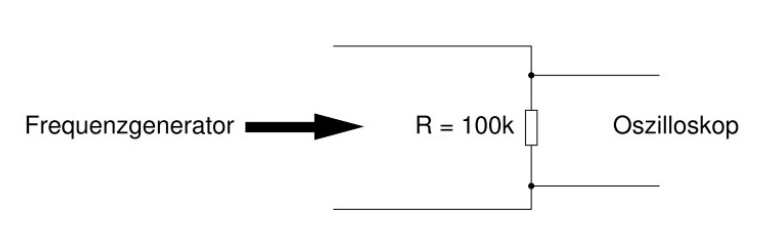
\includegraphics[width=100mm]{oszi_sg.png}
  \caption{Verbindung von Oszilloskop und Funktionsgenerator}
\end{figure}

\subsection{Durchführung}
Am Frequenzgenerator (Lastwiderstand \"High Z\") wird zuerst ein Dreieckssignal erzeugt. Dazu wird der Signaltyp \"Ramp\" ausgewählt, eine Freqzenz von $400Hz$ und eine Amplitude von $1V$ eingestellt, sowie die Symmetrie auf 50\% gesetzt (um den Sägezahn in ein Dreieck zu formen). Dann wird dem Dreieckssignal (mit Taste \"Mod\") ein Sinus mit Periodendauer $200\mu s$ ($f = \frac{1}{200\mu s} = 5kHz$) ("AM Freq") und Amplitude $100mV$ ("AM Depth") aufmoduliert. Die Schwingung wird am Oszilloskop dargestellt.

\subsection{Ergebnis}

\begin{figure}[H]
  \centering
  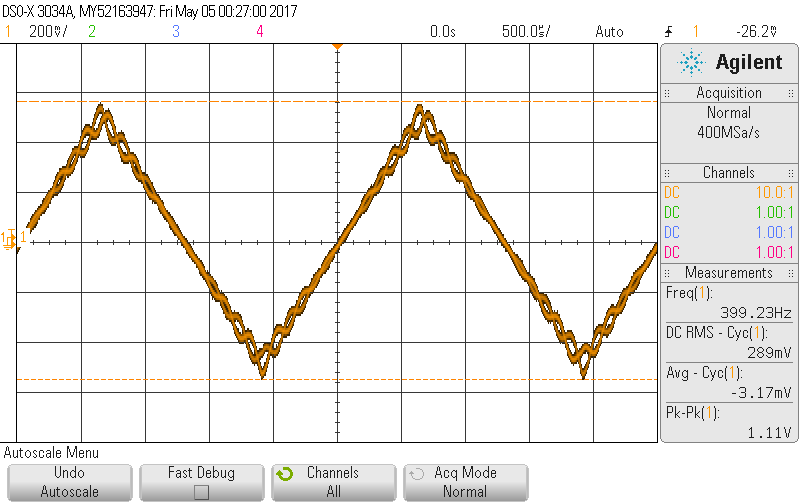
\includegraphics[width=150mm]{moduliertes_signal.png}
  \caption{Moduliertes Signal}
\end{figure}

\section{Diodenkennlinie}

\subsection{Aufgabenstellung}
Die Eigenschaften der Diode als nichtlineares Bauelement sollen in Form einer Kennlinier am Oszilloskop dargestellt werden.

\subsection{Verwendete Materialien und Einstellungen:}
\begin{itemize}
  \item Oszilloskop: Agilent InfiniiVision MSO-X 3054A
  \item Funktionsgenerator: Agilent 33220A
  \item Widerstand: $100\Omega$
  \item Dioden: LED rot, 1N4148
\end{itemize}

\subsection{Schaltungsaufbau}
\begin{figure}[H]
  \centering
  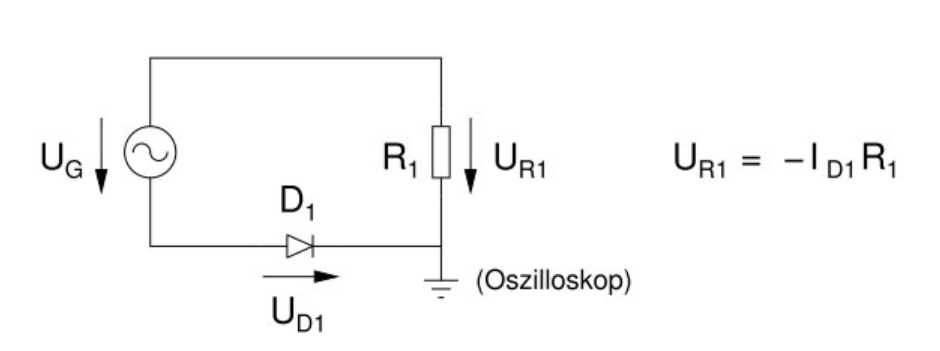
\includegraphics[width=150mm]{diodenschaltung.png}
  \caption{Diodenschaltung}
\end{figure}

\subsection{Durchführung}
Die Schaltung wird gemäß Plan zuerst mit einer roten LED und dann mit der 1N4148 Diode zur Vergleichsmessung in Serie mit einem $100\Omega$ Widerstand aufgebaut. Kanal 1 des Oszilloskops misst die Spannung an der Diode, Kanal 2 die Spannung am Widerstand (muss aufgrund der Position der Erdung invertiert geschalten werden). Das Oszilloskop befindet sich im XY-Betrieb, wodurch die Kennlinie sichtbar wird. Die Durchlassspannung wird mittels Cursor gemessen.

\subsection{Ergebnis}
Die Spannug wird mit Kanal 1 (X-Achse) an der Diode gemessen, der Strom mit Kanal 2 (Y-Achse) am Widerstand. Das Oszilloskop kann eigentlich nur Spannungen Messen, da der Strom jedoch über den Widerstand direkt proportional zur Spannung ist, kann dieser leicht berechnet werden. Um eine gute Darstellung der Kennlinie zu erreichen, muss eine geeignete Skalierung der Y-Achse eingestellt werden. Wenn die Durchlassspannung erreicht ist, kann viel Strom fließen.

\begin{figure}[H]
  \centering
  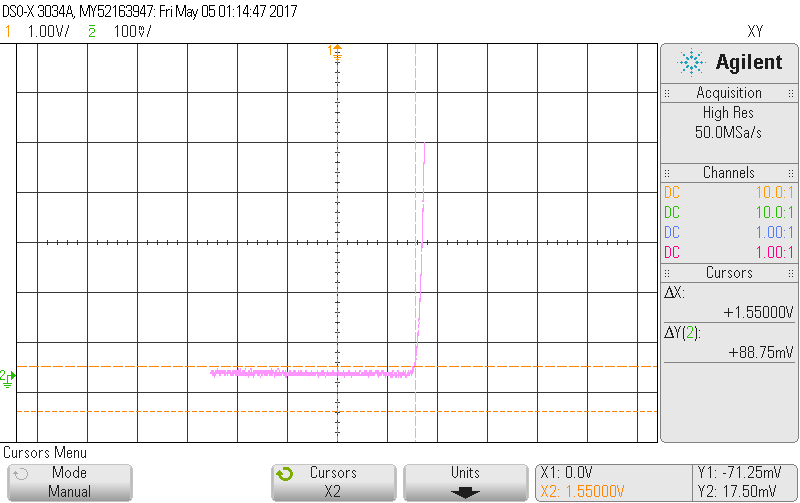
\includegraphics[width=150mm]{kennlinie_led.png}
  \caption{Kennlinie LED rot}
\end{figure}

Die Durchlassspannung der roten LED liegt laut Cursormessung bei $1,55V$. Diese ist etwas höher als bei \"herkömmlichen\" Dioden (siehe unten), da mit niedrigeren Spannungen kein sichtbares Licht erzeugt werden kann.

\begin{figure}[H]
  \centering
  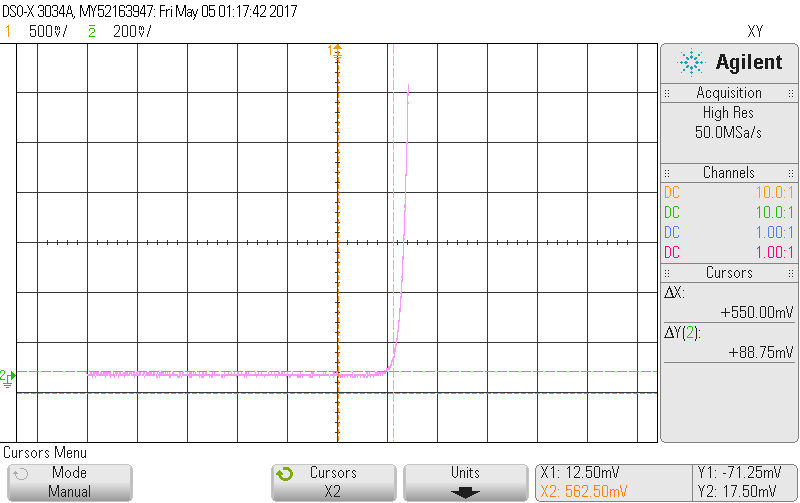
\includegraphics[width=150mm]{kennlinie_1n4148.png}
  \caption{Kennlinie 1N4148}
\end{figure}

Die Durchlassspannung der 1N4148 Diode liegt laut Cursormessung bei $0,55V$.

\end{document}
